


\begin{flushright}
\begin{footnotesize}
\textit{Von Olaf Radicke}
\end{footnotesize}
\end{flushright}
\smallskip

Das Werk \textit{"`No cross no crown"'} -- zu Deutsch: \textit{Ohne Kreuz keine
Krone} --
steht am Anfang der Quaker-Geschichte. Quasi mitten im
\textit{Quaker-Urknall}
um die 1660er Jahre. Aus dem Werk spricht die ganze Radikalität und
Aufbruchstimmung der jungen Glaubensgemeinschaft. Im Folgenden kann nur ein
Überblick über die weitere Entwicklung bis heute gegeben werden. Mir ist kein
deutscher Buchtitel bekannt, den ich dazu zur Vertiefung empfehlen kann. Im
Englischen wird man aber reichlich Material finden.

\medskip

Es gibt eine Reihe von Hypothesen wie oder warum das Quakertum
entstanden\index{Quaker!Ursprung} ist.
So
wollten einige im Quakertum einen Zweig der Mystik \index{Mystik} sehen.
Nachweislich ist, dass
sich Quaker mit der Mittelalter-Mystik beschäftigten\footnote{George Fox und die
Londoner Jahresversammlung standen der Mystik aber skeptisch bis ablehnend
gegenüber}, allerdings erst mit dem
Beginn der Kontakte zum Festland, durch ihre Missionierungsversuche
\index{Missionierung} unter
anderem in Holland \index{Orte:!Holland} und Deutschland
\index{Orte:!Deutschland}. Das war zu einem Zeitpunkt, wo die
theologischen Eckpfeiler für die Quaker schon ausformuliert waren. Also konnte
die Mystik nicht der Ursprung des Quakertums sein.

\medskip

Das Quakertum entstand aber nicht in einem luftleeren Raum und man kann Faktoren
nennen,
die zur Entstehung beitrugen. Das war zum einen die Übersetzung der Bibel
\index{Bibel!Übersetzung}
in die englische Sprache und der englische Bürgerkrieg
\index{Bürgerkrieg!englischer}. Ersteres befähigte auch
einfache Leute -- wie den Quaker George Fox \index{Personen:!Fox, George} -- zum
lesen der Bibel und somit zum
Errichten eines theologischen Gedankengebäudes, und letzteres sorgte für die
Verunsicherung und zum Teil Entmachtung der etablierten Kirchen
\index{Kirche!etablierte} und ihrer
Theologie. Es gab nicht mehr nur eine Kirche mit dem allein seligmachenden
Anspruch, sondern mehrere, die zu dem nicht mehr die enge Bindung zu einer
weltlichen Macht genoss.

\medskip

Viele Ideen, die wir im Quakertum finden, geisterten schon vorher durch die
Gesellschaft und Köpfe der zahllosen Splittergruppe, Sekten
\index{Sekte}, Suchenden und
Dissidenten \index{Dissident}, die in der Bürgerkriegszeit
\index{Bürgerkrieg} entstanden waren. Und das Quakertum
wäre höchstwahrscheinlich genauso wieder von der Bildfläche verschwunden wie
alle anderen auch, wenn es nicht die begnadeten Organisationstalente unter den
Quakern gegeben hätte. Natürlich wird auch einfach eine ordentliche Portion
Glück
dabei gewesen sein. Zu den -- heute noch allgemein bekannten --
Organisationstalenten gehörte George Fox, der die so genannten Monats-,
Vierteljahres-
und Jahres-Versammlungen \index{Jahresversammlung} \index{Monatsversammlung}
\index{Vierteljahresversammlung} organisierte, welche maßgeblich zu
funktionierenden
Strukturen beitrugen. Damit verbunden die etablierte "`Zucht des
Zusammenlebens"' \index{Zucht des Zusammenlebens}
--
Englisch: \textit{THE BOOK OF DISCIPLINE} \index{BOOK OF DISCIPLINE} . Also ein
\textit{Kirchenrecht} \index{Kirche!Kirchenrecht} welches
regelte, wie Dinge zu laufen haben. Ebenso wichtig war seine spätere Frau
Margaret Fell \index{Personen:!Fell, Margaret} (auch: \textit{Mother of
Quakerism} \index{Mother of Quakerism}). Während ihr späterer Mann
lange und oft im Gefängnis saß, war sie unermüdlich damit beschäftigt, die
gegenseitige Hilfe unter den Verfolgten \index{Verfolgung} Quakern zu
koordinieren. Ihr Anwesen
war in den ersten Jahren das Zentrum der Bewegung. Von hier aus wurden die
Missionsreisen organisiert, Seelsorge \index{Seelsorge} geleistet,
Rechtsbeistand geleistet und
politische Einflussnahme \index{Politik!Einflussnahme} geübt (das was man heute
\textit{Lobbyarbeit} \index{Lobbyarbeit} nennen
würde).

\medskip

William Penn ist für die Quaker in mehrfacher Weise von unschätzbarem Wert
gewesen.
Zum einen durch seine Kontakte in allerhöchste Kreise, durch seine adelige
Abstammung,
und
durch sein schriftstellerisches Wirken. Aber allen voran, wegen seinem so
genannten \textit{Heiligen Experiment}\index{Heilig!Heilige Experiment}, der
Gründung des Quakerstaates \index{Quaker!-staat} \index{Orte:!Pennsylvania}
Pennsylvania. Mit einem Schlag wurde aus einer kleinen \textit{Sekte von
Schwärmern und Ketzern} eine staatstragende soziale Gruppe. So haben die
damaligen Quaker noch bis heute sichtbare Spuren in den heutigen USA
\index{Orte:!USA}
hinterlassen.
Der damalige Quakerstaat wurde, auf Grund seiner liberalen Verfassung
\index{Verfassung}, die
rettende neue Heimat vieler wegen ihres Glaubens verfolgter Menschen. Das ist
auch der Grund, warum man bis heute noch bei Quakern zuerst an die USA denkt.

\medskip

Erst der \textit{Toleration Act} \index{Toleration Act} von 1689 beendete die
Verfolgung der Quaker im
Mutterland, der ihre Popularität und Verbreitung des Quakertums aber ohne hin
kaum eindämmen konnte.
 \index{Quaker!Verbreitung} 1660 gab
es in Britannien \index{Orte:!Britannien} und Irland \index{Orte:!Irland}
zusammen
66.000 Quaker, was etwa 0,76\% der
Gesamtbevölkerung war\footnote{P.Dandelion, "`Quakerism"', Seite 43, ISBN
0-521-60088-X}. Übertragen auf die heutige Bevölkerungsgröße wären das 492.684
Quaker. Heute sind es aber tatsächlich nur noch ungefähr
17.000\footnote{P.Dandelion, "`Quakerism"', Seite 178, ISBN 0-521-60088-X.}.

\medskip

William Penn verbrachte nur wenige Monate seines Lebens in Nordamerika
\index{Orte:!Nordamerika}. Die beiden
Quaker-Gruppen entwickelten sich auf Grund der geographischen Entfernung und den
politischen und sozialen Rahmenbedingungen unterschiedlich. In
England integrierten sich die Quaker nach dem \textit{Toleration Act} zusehends
in die Gesellschaft. Sie wurden \index{Wirtschaftliche!Erfolge} wirtschaftlich
erfolgreich und betätigten sich
auf den verschiedensten Gebieten, wie dem Bankwesen \index{Bankwesen}, der
Lebensmittelindustrie \index{Lebensmittelindustrie}
(bzw. Manufaktur) und der Schifffahrt. Ihre aufrührerischen und provokanten
Verhaltensweisen legten sie dabei zum Teil ab. So war es bald unüblich, die
Gottesdienste \index{Gottesdienst!stören} anderer Konfessionen
\index{Konfession} zu stören. Das Abnehmen des Hutes und die
Verwendung von Ehrentiteln wurden aber weiterhin abgelehnt.

\medskip

Im achtzehnten Jahrhundert lebten die Quaker zurückgezogen.
Universitäten \index{Universität} und der akademische Betrieb waren verpönt.
\index{Theater} Theater, Tanz \index{Tanz} und Musik \index{Musik}
wurden weiterhin abgelehnt. Geheiratet \index{Heirat} wurde nur innerhalb der
Glaubensgemeinschaft. Die Kleidung \index{Kleidung} war schmucklos und in
gedeckten Farben
(zumeist Grau) gehalten. Die Missionstätigkeit wurde weitestgehend eingestellt.
Theologische Auseinandersetzungen fanden zumeist nur innerhalb der Gemeinschaft
statt. Dann aber zum Teil umso heftiger. Ein ersten Auftakt bildete schon die
\textit{Keith-Kontroverse} \index{Keit-Kontroverse}, die schon zu einem
stehenden Begriff geworden ist und sogar schon am Ende des zibzehnen Jahrhundert
vom Zaun brach. George Keith (1638/9 -- 1716) \index{Personen:!Keith, George}
war schottischer
Quaker und Missionar, der in
Nordamerika tätig war und durch seine Ansichten für heftige Kontroversen
sorgte. Und auch hierbei ging es schon um die Frage zur Nähe zur Bibel und die
Bedeutung von tradituenellen Christlichen Positionen.

\medskip

In Nordamerika wurden die Quaker ebenfalls wirtschaftlich sehr erfolgreich. Dort
sind sie untrennbar mit dem Walfang \index{Walfang} verbunden. In
\textit{Moby-Dick} setzt
Herman Melville \index{Personen:!Melville, Herman} dem blutigen Gewerbe ein
literarisches Denkmal, wenn man so
will. Auch dieses Werk trug zum allgemeinen Bild der Quaker bei.

\medskip

Aber es gab auch andere Gebiete neben der Wirtschaft, in denen sich Quaker noch
einen
Namen gemacht haben. So in der Sklaven-Frage \index{Sklaverei}. Nur fünf Jahre
nach Eintreffen
der ersten deutschen Quaker in Pennsylvania initiierte Franz Daniel Pastorius
\index{Personen:!Pastorius, Franz Daniel}
1688 \textit{Germantown Quaker Petition Against Slavery}
\index{Orte:!Germantown}\footnote{Wikipedia,
\\The 1688 Germantown Quaker Petition Against Slavery,
\\http://en.wikipedia.org/wiki/The\_1688\_Germantown\_Quaker\_Petition\_Against\
\_Slavery.} Das Thema Sklaverei wird die Quaker die nächsten fast 100 Jahre
nicht
loslassen. Erst 1758 beschloss Philadelphia \index{Orte:!Philadelphia} als erste
Jahresversammlung ein Verbot der Sklaverei,
unter Androhung des Ausschlusses ihrer eigenen Mitglieder.

\medskip

Auch in Britannien kämpften die Quaker um diese Zeit gegen die Sklaverei.
Allerdings nicht in ihren eigenen Reihen, sondern gegen die Hersteller
und Händler von Produkten der Sklavenbesitzer. Also zum Teil gegen ihre
Glaubensbrüder in Nordamerika. Den Quakern in Britannien darf wohl zugestanden
werden, in diesem Zusammenhang sogar die Erfinder des Produkt-Boykotts
\index{Boykott} zu sein.
Sie zogen durch das Land und hielten Vorträge über Sklaverei, um so Konsumenten
zu
bewegen, keine Produkte zu kaufen, die mit Sklaverei zu tun hatte. Und sie
waren überaus erfolgreich dabei. Was bedeutet, dass sie einige Profiteure der
Sklaverei in den Ruin trieben.

\medskip

Aber auch in Nordamerika \index{Orte:!Nordamerika} scheuten einige Quaker nicht
davor zurück,
Sklavenbesitzern unmittelbar Schaden an ihrem \textit{Eigentum} zuzufügen, indem
sie sich
aktiv an Sklavenbefreiungen beteiligten. Die sogenannte
\textit{Underground Railroad} \index{Underground Railroad} war ein
ausgeklügeltes System von Fluchthelfern. Das
Besondere dabei war, dass jeder Fluchthelfer \index{Fluchthelfer}
immer
nur einen Knotenpunkt in einem
Netzwerk darstellte. Wenn ein Knoten ausfiel, konnte er durch andere ersetzt
werden. Das macht das System sehr robust gegen Störungen. Heute würde man
wohl
von einem \textit{Peer-to-Peer-Netzwerk} sprechen.

\medskip

Auch wenn das \textit{Heilige Experiment}, also der Quakerstaat in Pennsylvania,
nur achtzig Jahre
bestanden hatte\footnote{Immerhin! Die Täufer im Neuen Jerusalem (Münster)
\index{Orte:!Jerusalem!neues} \index{Orte:!Münster} haben
nicht mal zwei Jahre durchgehalten.}, so verlief die weitere
Quakergeschichte in Nordamerika wesentlich interessanter als in der
\textit{Alten
Welt} -- Europa. Die Missionierungsversuche \index{Missionierung} der britischen
Quaker in
\textit{Europa} \index{Orte:!Europa} -- also dem Festland, blieben ohne
langfristigen Erfolg.
Entweder waren ihre Verfolger \index{Verfolgung} und Feinde so erbarmungslos,
dass eine
Konversion einem Todesurteil gleich kam, so zumeist in den katholischen
\index{Orte:!katholischen Ländern}
Ländern, die von den Quakern \textit{dark countries} -- also: Länder der
Finsternis -- genannt wurden, oder es gab innergemeinschaftliche Probleme.
Gerade
für junge Männer war es attraktiver, als konvertierter Quaker nach Nordamerika
auszuwandern als sich mit den Sorgen und Nöten der \textit{Alten Welt} herum
zu
schlagen. Gerade auch im Hinblick auf Heiratschancen \index{Heirat}. In den
kleinen
Gemeinschaften auf dem europäischen Festland war die Wahl in der eigenen
Gemeinschaft sehr begrenzt und die Heirat außerhalb der Gemeinschaft war (noch)
nicht erlaubt. Und so missionierten die britischen Quaker indirekt für
Nordamerika.

\medskip

Typisch für die nordamerikanische Quaker-Geschichte waren die zahlreichen
Spaltungen. Die erste Spaltung \index{Spaltung} entzündete sich anlässlich des
Amerikanischen
Unabhängigkeitskriegs an der Frage des Friedenszeugnises
\index{Friedenszeugnis}. Die meisten Quaker
standen fest zu der Überzeugung, sich an keinem Krieg \index{Krieg} zu
beteiligen. Einige
wenige hielten das Friedenszeugnis für entbehrlich und spalteten sich zu den
\index{Freien Quaker} \index{Quaker!Freie} ab,
die sich dann am Unabhängigkeitskrieg \index{Unabhängigkeitskrieg}
beteiligten. Dieser Zweig starb 1834 aus. Die nächste größere Spaltung war die
der Ann Lee \index{Personen:!Lee, Ann}. Deren Abspaltung -- die sich theologisch
völlig verselbständigte --
wurde \textit{Shaker} \index{Shaker} genannt. Den Höhepunkt hatte
diese Bewegung in der Mitte
des 19. Jahrhunderts.

\medskip

Zu Beginn des 19. Jahrhunderts kam es zu einer anderen Spaltung, die das
Quakertum in zwei Lager teilte.
In die \textit{Hicksites} \index{Quaker!Hicksites} und die
\textit{Orthodox
Friends} \index{Quaker!Orthodox Friends}. Im Gegensatz zu der Shaker-Spaltung,
beanspruchten beide weiter für
sich, das \textit{wahre Quakertum} zu vertreten. Der Streit entzündete sich an
der Person von Elias Hicks (1748 -- 1830) \index{Personen:!Hicks, Elias}.
Deshalb
auch der Name \textit{Hicksites}.
Hicks war seit seinem 27. Lebensjahr von seiner Andachtsgemeinschaft als
Prediger
anerkannt. Er war Abolitionist \index{Abolitionist}, also Kämpfer
für die Sklavenbefreiung. Auch
organisierte er Produkt-Boykotts von unter Sklaverei produzierten Waren. In dem
Konflikt ging es vermutlich nicht nur um theologische Fragen, sondern
unterschwellig auch um die Antipathie zwischen den ländlichen und den urbanen
Quakern. Die theologische Kontroverse drehte sich um die Frage, ob Jesus
göttlicher Natur sei, ob die Errettung nur durch den Opfertod Jesus möglich ist
und ob das innere Licht \index{Licht!Inneres} -- also die innere Offenbarung --
über der Bibel \index{Bibel} stehe.
Die Gegner warfen Hicks Häresie vor und unterstellten ihm, von zentralen
Aussagen des Christentums abzuweichen. Hicks ist in der quietistischen
 Tradition
von John Woolman \index{Personen:!Woolman, John} und Job Scott
\index{Personen:!Scott, Job} zu sehen. Seine Gegner, die \textit{Orthodox
Friends} \index{Quaker!Orthodox Friends} vertraten quakerfremde christliche
Traditionen. Die
\textit{Orthodox Friends} störten sich auch an der Position von Hicks, der nicht
an einen Teufel \index{Satan} glaubte, der das Böse zu den Menschen
brächte, sondern er
glaubte, dass die Leidenschaft (im negativen Sinne) ein Teil der menschlichen
Natur sei, und das die Sünde \index{Sünde} somit im Menschen ist. 1827 spaltete
sich die
Philadelphia-Jahresversammlung und es gab auf einmal zwei Jahresversammlungen,
die von sich behaupteten \textit{die} echte Philadelphia-Jahresversammlung zu
sein.
Ihr folgten dann in den nächsten Jahren New York \index{Orte:!New York},
Baltimore \index{Orte:!Baltimore}, Ohio \index{Orte:!Ohio} und
Indiana \index{Orte:!Indiana}.

\medskip

Ein paar Jahre später (1843) kam es dann im \textit{Orthodox Friends}-Flügel
noch mal zu einer Aufspaltung, zur Gurneyite-Wilburite-Spaltung
\index{Gurneyite-Wilburite-Spaltung}. Die beiden
Kontrahenten waren diesmal John Wilbur (1774 -- 1856) \index{Personen:!Wilbur,
John} und Joseph John Gurney
(1788 -- 1847) \index{Personen:!Gurney, John}. Gurney war Brite, Bankier
\index{Personen:!Bankier} und Bruder von Elizabeth Fry \index{Personen:!Fry,
Elizabeth}, die für
ihre Gefängnisarbeit \index{Gefängnis!Gefängnisarbeit} und ihr Eintreten gegen
die Todesstrafe \index{Todesstrafe} bekannt werden
sollte und auf ihren Missionsreisen bis nach Berlin\index{Orte:!Berlin} kam.
Er war auch Prediger \index{Personen:!Prediger} und in dieser Funktion
von seiner
Versammlung autorisiert (im englischen \textit{recorded Quaker minister}). Als
Gurney auf seiner Reise in Nordamerika predigte, kritisierte er, das unter den
Quakern die Bibel \index{Bibel} vernachlässigt würde, und er betonte den Glauben
an die
Rettung durch den Glauben an Christus. Somit vertrat er traditionelle
protestantische Theologie \index{Theologie!protestantische}. Aus seinen
Anhängern, die \textit{Gurneyite Quakers}
genannt wurden, spalteten sich später die evangelikalen Quaker
\index{Quaker!Evangelikal} ab.

\medskip

Wilbur war in Rhode Island \index{Orte:!Rhode Island} geboren worden, also
Nordamerikaner. Er reiste seinerseits
nach Britannien und bemerkte, dass die dortigen Quaker nach dem Hicksite-Schisma
in seinen Augen über das Ziel hinaus schossen, in dem sie die Bibel nun
überbetonten, und das \textit{Innere Licht} durch Rationalismus drohte verdrängt
zu werden. Wilbur zitierte wieder die frühen Freunde Robert Barclay
\index{Personen:!Barclay, Robert}, William
Penn und George Fox \index{Personen:!Fox,
George}, um an die Basis des Quakertums zu erinnern. Auch wenn er
nach wie vor nicht in Zweifel zog, dass die Bibel durch Gott inspiriert war und
ein Leitfaden der frühen Quaker darstellte. Die Anhänger von Wilbur wurden
\textit{Wilburites} genannt. Sie waren zu den
\textit{Gurneyite Quakers} deutlich in der Minderzahl.
Aus den \textit{Wilburites} sollte später die
\textit{Conservative Friends} \index{Quaker!Conservative Friends} -- also die
\textit{Konservativen Quaker} --
hervorgehen.

\medskip

In den nächsten Jahren gab es dann noch zahlreiche kleinere Spaltungen,
Umbenennungen, Neugründungen und Wiedervereinigungen, wie zum Beispiel die
\textit{Beanite Qaker} \index{Quaker!Beanite}, die \textit{Nontheist
Friends} \index{Quaker!Nontheist Friends}, das \textit{Quaker Universalist
Fellowship} \index{Quaker!Universalist Fellowship}, das \textit{New
Foundation Fellowship} \index{Quaker!New Foundation Fellowship}, die
\textit{Richmond Declaration} \index{Richmond Declaration}, das \textit{Five
Years Meeting}, das \textit{Evangelical Friends International}
\index{Quaker!Evangelical Friends}, das \textit{Friends United
Meeting} \index{Quaker!Friends United Meeting}, die \textit{Friends General
Conference} \index{Quaker!Friends General Conference} und das \textit{Friends
World Committee for Consultation} und so weiter... Wo man so schnell auch nicht
durchblickt.
Die äußerlichen Erkennungsmerkmale, wie die \textit{Quaker!-Uniform}
\index{Quaker!Uniformem} und der Quakerhut, wurden
langsam ausrangiert. Je nach Quaker-Zweig früher oder etwas später. Im 20.
Jahrhundert waren sie dann weitestgehend verschwunden. Es wurde noch weiterhin
auf
nicht allzu dekadentes Auftreten geachtet, aber ansonsten passte man sich
optisch weitestgehend der Gesellschaft an. Die evangelikalen Quaker begannen
sogar in ihren Versammlungen zu singen, zu taufen, Abendmahl zu feiern,
richteten Pastoren-Ämter ein und nannten
fortan ihrer Versammlungshäuser \textit{Kirchen} \index{Kirche!Bezeichnung}
(englisch: \textit{church}),
ein Begriff gegen den die Frühen Freunde gewettert hatten. Auch in "`Ohne Kreuz
keine Krone"' machte William Penn klar, das die Kirche die \textit{Gemeinschaft
der
Gläubigen} war, und nicht ein Gebäude aus Holz oder Stein. George Fox
verspottete
die "`Gotteshäuser"' der "`Namenschristen"' gar als
"`Turmhäuser"'\index{Kirche!Turmhaus}, wegen ihrer
Glockentürme. Bis heute hat sich der evangelikale Flügel des Quakertums soweit
den konventionellen protestantischen Kirchen angenähert, dass es kaum noch
einen
erkennbaren Unterschied gibt. Aber dieser Zweig war der am schnellsten
wachsende!

\medskip

Zum Beginn des 20. Jahrhundert steckte das Quakertum in einer Identitätskrise.
Es gab kaum mehr neue Impulse, weder von Außen
noch von Innen. Das Quakertum war
nach Innen und nach Außen immer weniger attraktiv geworden. Dann brachen die
beiden Katastrophen -- der Erste und der Zweite Weltkrieg\index{Weltkrieg} --
über die Welt
herein. In dieser Zeit erhob sich auf einmal das Friedenszeugnis
\index{Friedenszeugnis}\textit{wie
Phönix aus der Asche}. Allen voran war es Rufus Matthew Jones,
\index{Personen:!Jones, Rufus Matthew} dem
es gelang, die heillos zerstrittenen Quaker-Flügel wieder unter der Flagge des
Friedenszeugnises zu vereinen. Das Friedenszeugnis war auf einmal ein
gemeinsamer Identitätsstifter. Gerade Deutschland
\index{Orte:!Deutschland} profitierte von der Hilfe der
Quaker. Vermutlich wurden tausende Kinder nach dem Ersten und Zweiten Weltkrieg
durch die Quakerspeisung \index{Quaker!Speisung} vor dem Verhungern gerettet.
Zwischen den Weltkriegen
wurden bei den sogenannten \textit{Kinder!-transporten}
\index{Kinder!-transporten}
tausende jüdische Kinder \index{Kinder!jüdisch}
vor der Vernichtungsmaschinerie der Nazis gerettet. In beiden Weltkriegen war es
für Quaker bestimmt nicht immer leicht, sich gegen einen
angeblich \textit{"`gerechten"'}
Krieg zu stellen. Und bis heute kann man darüber diskutieren, ob es richtig
war, dass die Quaker sich weigerten, die Waffen gegen Nazi-Deutschland zu
ergreifen.

\medskip

In der zweiten Hälfte des 20. Jahrhunderts wurde das Quakertum quasi auf den
Kopf
gestellt. Hatten noch 1940 die meisten Quaker auf der Nordhalbkugel der Erde
gewohnt, so gab es im Jahre 2000 mehr, die auf der Südhalbkugel lebten:

\begin{center}
\begin{tabular}{|l|r|r|} \hline
                        & \textbf{1940}        & \textbf{2000}    \\ \hline
\hline
Nordamerika             & 112.300              & 92.300           \\ \hline
Europa                  & 22.600               & 19.100           \\ \hline
\textbf{Nordhalbkugel}  & \textbf{134.900}     & \textbf{111.400} \\ \hline
Afrika                  & 13.200               & 156.200          \\ \hline
Mittel/Südamerika       & 7.200                & 60.600           \\ \hline
\textbf{Südhalbkugel}   & \textbf{20.400}      & \textbf{216.800} \\ \hline
\end{tabular}
\end{center}


Da die evangelikalen Quaker in erster Linie in der Mission tätig waren, ist es
auch so, dass die meisten Quaker auf der Südhalbkugel (und somit auf der Welt)
evangelikale Quaker sind.

% \section{Persönliches Resümee}
% 
% Der Grund, warum das deutsche Quakertum in dem obigen Text kaum vorkam, ist der,
% dass sie für Gesamtquakertum, das deutsche Quakertum \index{Quaker!Quakertum in
% Deutschland} weder quantitativ noch
% qualitativ eine Rolle gespielt hat oder spielt. Das Quakertum konnte sich im
% deutschsprachigen Raum nie dauerhaft etablieren, noch hat es theologische
% Impulse
% über die Grenzen von Deutschland hinaus gegeben. Das hatte verschiedenste
% Gründe, über die man ein eigenes Buch füllen kann.
% % Claus, das wird an dir höngen bleiben! Hast du schon angefangen
% % damit??
% Im jedem Fall denke ich, dass
% ich dem deutschen Quakertum kein Unrecht antut, wenn ich sage, dass es nie
% repräsentativ für das gesamte Quakertum war. Bis zum heutigen Tag. Ich denke, es
% ist schon schwer genug, das Wesentliche vom Quakertum erkennen und verstehen zu
% können, so dass ich den Blick nicht unnötig ablenken wollte, durch die
% Besonderheiten des deutschsprachigem Quaertums\footnote{"`deutschsprachigem
% Quaertums"' deshalb,
% weil ich Österreich dazu zähle.}.
% Es gab immer wieder einzelne
% Persönlichkeiten in Deutschland, die durchaus nachhaltige Spuren hinterlassen
% haben. So
% zum Beispiel Ludwig Seebohm\index{Personen:!Seebohm, Ludwig}. Auf
% Seite~\pageref{ref:l_seebohm} geht Claus Bernet
% auf ihn ausführlicher ein.
% 
% \medskip
% 
% Doch zurück zum "`Welt-Quaker-Mainstream"'\index{Quaker!Mainstream}, wenn man so
% will: Erinnern wir uns noch Mal
% an das oben gesagte. Ich bin nicht allzusehr auf theologische Details
% eingegangen. Mir wurde gesagt "`geht doch bitte noch mal darauf ein, was
% Quakertum an sich ausmacht und was das Besondere daran ist."' Das ist wirklich
% nicht so einfach. Ich würde die Entwicklung des Quakertums mit einem
% Brennglas\index{Brennglas}
% vergleichen: Auf der einen Seite kommen verschiedenste Impulse und Ideen herein
% und werden gebündelt. So war die Idee des "`Inneren
% Lichts"'\index{Licht!Inneres} schon vor
% George Fox\index{Personen:!Fox, George} im Umlauf und wurde unter anderem von
% Anne Hutchinson\index{Personen:!Hutchinson, Anne} propagiert.\footnote{Aber auch
% andere quakertypische Elemente lassen sich schon vorher finden:
% \textbf{Stille Andacht} Im letzten Absatz des 14. Abschnitts im 5. Kapitel
% (Seite~\pageref{kap5_ab14} bis \pageref{ref:05_13_zurueckgezogenheit_ende}) lobt
% William Penn die Zurückgezogenheit, die auch die katholische Kirche kennt.
% \textbf{Gleichheit} wurde auch schon zuvor von den True Levellers propagiert.
% \textbf{Ablehnung eines Klerus} war schon von den Täufern bekannt.
% \textbf{Konsensentscheidungen} waren schon 400 v.Ch. bei buddhistischen Mönchen
% üblich.
% \textbf{Kriegsdiensverweigerung} war ebenfalls von Täufern bekannt.
% \textbf{Frauen als Predigerinnen} gab es auch schon vor den Quäkern.
% \textit{"`...Was da ist, war längst, und was sein wird, ist längst gewesen; und
% Gott sucht das Entschwundene wieder hervor."'} -- Der Prediger Salomo, Kapitel
% 3,15
% } In der
% Quakerbewegung wurden verschiedenste Elemente zu einem neuen Konglomerat
% gebündelt, was sich als tragfähig und erfolgreich herausstellten.
% So wie das Licht, wenn
% es den Brennpunkt der Linse erreicht hat. Und so, wie sich das Licht dann hinter
% dem Brennpunkt wieder (über Kreuz) auffächert, so spalteten sich die
% verschiedenen Quaker-Flügel\index{Quaker!-Flügel} wieder auf, weil sie glaubten
% den einen oder anderen Aspekt betonen zu müssen und das Eine oder Andere für
% entberlich hielten. Der durch die Linse zuvor gebündelte
% Lichtstrahl streut immer mehr, um so weiter es sich von dem
% Brennpunkt der Linse entfernt hat. Bis das Licht seine Intensitiät soweit
% eingebüßt hat, dass es sich von seiner Umgebung kaum mehr abgesetzt und wahrnehmbar
% ist. An diesem
% Punkt befindet sich das Quakertum heute. Das Spektrum reicht von Nontheisten,
% für die
% es keinen Gott mehr braucht, bis zu
% Evangelikal-Bibelzentrische\index{Quaker!Bibelzentrismus}
% \index{Quaker!Evangelikal}, die jedem das
% Seelenheil absprechen, der nicht getauft\index{Taufe} ist und sich zu
% Jesus Christus
% bekennt. Quakertum wird so kaum mehr fassbar. Quakertum scheint heute alles und
% irgend wir auch wieder nichts zu sein.
% 
% \begin{center}
% % Graphic for TeX using PGF
% Title: /home/or/PRVATE-OPT/q/quaeker/eigene_texte/git_repos_no_cross/no_cross_no_crown_de/brennpunkt.dia
% Creator: Dia v0.97
% CreationDate: Sat Oct 3 20:30:27 2009
% For: or
% \usepackage{tikz}
% The following commands are not supported in PSTricks at present
% We define them conditionally, so when they are implemented,
% this pgf file will use them.
\ifx\du\undefined
 \newlength{\du}
\fi
\setlength{\du}{15\unitlength}
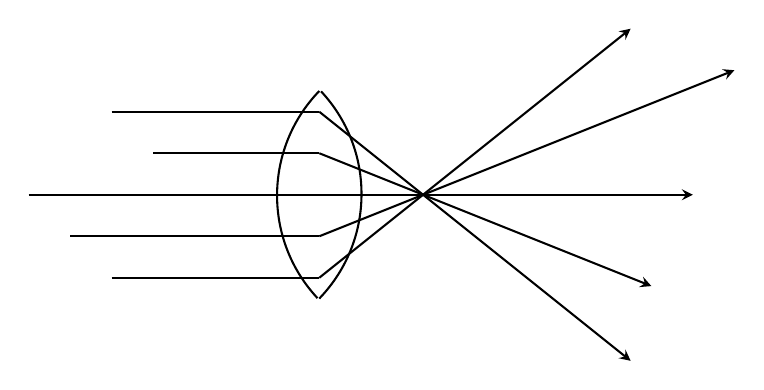
\begin{tikzpicture}
\pgftransformxscale{1.000000}
\pgftransformyscale{-1.000000}
\definecolor{dialinecolor}{rgb}{0.000000, 0.000000, 0.000000}
\pgfsetstrokecolor{dialinecolor}
\definecolor{dialinecolor}{rgb}{1.000000, 1.000000, 1.000000}
\pgfsetfillcolor{dialinecolor}
\pgfsetlinewidth{0.050000\du}
\pgfsetdash{}{0pt}
\pgfsetdash{}{0pt}
\pgfsetbuttcap
{
\definecolor{dialinecolor}{rgb}{0.000000, 0.000000, 0.000000}
\pgfsetfillcolor{dialinecolor}
% was here!!!
\definecolor{dialinecolor}{rgb}{0.000000, 0.000000, 0.000000}
\pgfsetstrokecolor{dialinecolor}
\pgfpathmoveto{\pgfpoint{5.000100\du}{2.499895\du}}
\pgfpatharc{224}{137}{3.625000\du and 3.625000\du}
\pgfusepath{stroke}
}
\pgfsetlinewidth{0.050000\du}
\pgfsetdash{}{0pt}
\pgfsetdash{}{0pt}
\pgfsetbuttcap
{
\definecolor{dialinecolor}{rgb}{0.000000, 0.000000, 0.000000}
\pgfsetfillcolor{dialinecolor}
% was here!!!
\definecolor{dialinecolor}{rgb}{0.000000, 0.000000, 0.000000}
\pgfsetstrokecolor{dialinecolor}
\pgfpathmoveto{\pgfpoint{4.999769\du}{7.500243\du}}
\pgfpatharc{44}{-43}{3.625000\du and 3.625000\du}
\pgfusepath{stroke}
}
\pgfsetlinewidth{0.050000\du}
\pgfsetdash{}{0pt}
\pgfsetdash{}{0pt}
\pgfsetbuttcap
{
\definecolor{dialinecolor}{rgb}{0.000000, 0.000000, 0.000000}
\pgfsetfillcolor{dialinecolor}
% was here!!!
\definecolor{dialinecolor}{rgb}{0.000000, 0.000000, 0.000000}
\pgfsetstrokecolor{dialinecolor}
\draw (0.000000\du,3.000000\du)--(5.000000\du,3.000000\du);
}
\pgfsetlinewidth{0.050000\du}
\pgfsetdash{}{0pt}
\pgfsetdash{}{0pt}
\pgfsetbuttcap
{
\definecolor{dialinecolor}{rgb}{0.000000, 0.000000, 0.000000}
\pgfsetfillcolor{dialinecolor}
% was here!!!
\definecolor{dialinecolor}{rgb}{0.000000, 0.000000, 0.000000}
\pgfsetstrokecolor{dialinecolor}
\draw (-2.000000\du,5.000000\du)--(5.000000\du,5.000000\du);
}
\pgfsetlinewidth{0.050000\du}
\pgfsetdash{}{0pt}
\pgfsetdash{}{0pt}
\pgfsetbuttcap
{
\definecolor{dialinecolor}{rgb}{0.000000, 0.000000, 0.000000}
\pgfsetfillcolor{dialinecolor}
% was here!!!
\definecolor{dialinecolor}{rgb}{0.000000, 0.000000, 0.000000}
\pgfsetstrokecolor{dialinecolor}
\draw (0.000000\du,7.000000\du)--(5.000000\du,7.000000\du);
}
\pgfsetlinewidth{0.050000\du}
\pgfsetdash{}{0pt}
\pgfsetdash{}{0pt}
\pgfsetbuttcap
{
\definecolor{dialinecolor}{rgb}{0.000000, 0.000000, 0.000000}
\pgfsetfillcolor{dialinecolor}
% was here!!!
\pgfsetarrowsend{stealth}
\definecolor{dialinecolor}{rgb}{0.000000, 0.000000, 0.000000}
\pgfsetstrokecolor{dialinecolor}
\draw (5.000000\du,7.000000\du)--(12.500000\du,1.000000\du);
}
\pgfsetlinewidth{0.050000\du}
\pgfsetdash{}{0pt}
\pgfsetdash{}{0pt}
\pgfsetbuttcap
{
\definecolor{dialinecolor}{rgb}{0.000000, 0.000000, 0.000000}
\pgfsetfillcolor{dialinecolor}
% was here!!!
\pgfsetarrowsend{stealth}
\definecolor{dialinecolor}{rgb}{0.000000, 0.000000, 0.000000}
\pgfsetstrokecolor{dialinecolor}
\draw (5.000000\du,5.000000\du)--(14.000000\du,5.000000\du);
}
\pgfsetlinewidth{0.050000\du}
\pgfsetdash{}{0pt}
\pgfsetdash{}{0pt}
\pgfsetbuttcap
{
\definecolor{dialinecolor}{rgb}{0.000000, 0.000000, 0.000000}
\pgfsetfillcolor{dialinecolor}
% was here!!!
\pgfsetarrowsend{stealth}
\definecolor{dialinecolor}{rgb}{0.000000, 0.000000, 0.000000}
\pgfsetstrokecolor{dialinecolor}
\draw (5.000000\du,3.000000\du)--(12.500000\du,9.000000\du);
}
\pgfsetlinewidth{0.050000\du}
\pgfsetdash{}{0pt}
\pgfsetdash{}{0pt}
\pgfsetbuttcap
{
\definecolor{dialinecolor}{rgb}{0.000000, 0.000000, 0.000000}
\pgfsetfillcolor{dialinecolor}
% was here!!!
\pgfsetarrowsend{stealth}
\definecolor{dialinecolor}{rgb}{0.000000, 0.000000, 0.000000}
\pgfsetstrokecolor{dialinecolor}
\draw (5.000000\du,6.000000\du)--(15.000000\du,2.000000\du);
}
\pgfsetlinewidth{0.050000\du}
\pgfsetdash{}{0pt}
\pgfsetdash{}{0pt}
\pgfsetbuttcap
{
\definecolor{dialinecolor}{rgb}{0.000000, 0.000000, 0.000000}
\pgfsetfillcolor{dialinecolor}
% was here!!!
\definecolor{dialinecolor}{rgb}{0.000000, 0.000000, 0.000000}
\pgfsetstrokecolor{dialinecolor}
\draw (-1.000000\du,6.000000\du)--(5.000000\du,6.000000\du);
}
\pgfsetlinewidth{0.050000\du}
\pgfsetdash{}{0pt}
\pgfsetdash{}{0pt}
\pgfsetbuttcap
{
\definecolor{dialinecolor}{rgb}{0.000000, 0.000000, 0.000000}
\pgfsetfillcolor{dialinecolor}
% was here!!!
\definecolor{dialinecolor}{rgb}{0.000000, 0.000000, 0.000000}
\pgfsetstrokecolor{dialinecolor}
\draw (1.000000\du,4.000000\du)--(5.000000\du,4.000000\du);
}
\pgfsetlinewidth{0.050000\du}
\pgfsetdash{}{0pt}
\pgfsetdash{}{0pt}
\pgfsetbuttcap
{
\definecolor{dialinecolor}{rgb}{0.000000, 0.000000, 0.000000}
\pgfsetfillcolor{dialinecolor}
% was here!!!
\pgfsetarrowsend{stealth}
\definecolor{dialinecolor}{rgb}{0.000000, 0.000000, 0.000000}
\pgfsetstrokecolor{dialinecolor}
\draw (5.000000\du,4.000000\du)--(13.000000\du,7.200000\du);
}
\end{tikzpicture}



% \end{center}
% 
% \medskip
% 
% Der Punkt der höchsten Konzentration und "`Reinheit"' des Quakertums -- also dem
% Brennpunkt um beim Bild zu bleiben -- war der, wo William Penn "`Ohne Kreuz
% keine Krone"' geschrieb. Wenn der Leser also diese Buch gelesen hat, wird er die
% zentralen
% Anliegen der frühen Quaker kennen. Welch der heute existierenden Quaker-Flügel
% seiner Meinung nach, noch die ursprüngliche Quakeridee repräsentiert oder auch
% nicht, das über lasse ich dem Leser. Eine Frage, die wir uns aber kaum entziehen
% können ist, ob der radikale Ton den William Penn in seinem Buch "`Ohne Kreuz
% keine Krone"' anschlägt, heute noch "`Mehrheitsfähig"' währe. Die Gegenfrage
% währe,
% ob denn einen Quakertum "`mehrheitsfähig"' sein muss? Oder: Ob der radikale Ton
% den William Penn "`mehrheitsfähig"' sein muss?
% Es gibt einige Stell, wo auch
% ich so meine Probleme habe. Wenn etwa auf Seite~\pageref{kap15_ab5} für
% Frauen andere Freizeitbeschäftigungen vorgeschlagen werden, als für Männer. Oder
% wenn auf Seit~\pageref{ref:haarflechten} gesagt wird, das Frauen die sich die
% Haare flechten, keine \textit{Gottseligkeit} zu erwarten hätten. Also, wo
% betrachtet man berechtigter Weise Dinge als Irrtum und wo biegt man sich das
% Quakertum zu seiner Bequemlichkeit zurecht? Die Fragen ist so alt, wie das
% Quakertum selbst. Und jede Generation muss sie für sich neu beantworteten.
% 
% \medskip
% 
% Ich glaube wenn es etwas gibt im Quakertum, was ununterbrochen bestand hatte und
% Charakteristisch ist, dann die Streitkultur. Es wurde immer und oft heftig unter
% Quakern gestritten. Es wurde ausgestossen, gespalten, wiedervereint und
% wiederaufgenommen, aber es wurden nie Scheiterhaufen errichtet. Weder für Quaker
% noch für Nichtquaker. Es gab nur eine kurze Zeit, in der Quaker sich
% weitestgehend
% einig waren, und den Rest der Welt für den Unglauben in ihr -- oder
% \textit{Aberglaube} wie es bei William Penn heisst -- kollektiv anklagten. Das
% wird immer wieder deutlich, wenn William Penn in dem hier vorliegenden Text,
% davor warnt \textit{"`sich mit
% der Welt ein zu lassen"'}. Nur zu diesem Zeitpunkt verlief die "`Frontliene"'
% zwischen den den Quakern -- als geschlossene Gruppe -- einerseitz, und der rest
% der "`Welt"' anderereseits. Spähter, mit den inneren (Dauer-)Konflikten,
% wanderte der Fokus
% nach Innen. Eine Mission nach aussen fand nicht -- oder kaum mehr -- statt.
% Irgend wann hiess es dann "`Quaker missionieren nicht"'. Nun, ich glaube da hat
% man die Not zur Tugend erklärt. Der jüngste Evangelikale-Flügel missioniert
% wieder und das überaus erfolgreich, wie ich oben schon an Hand der Zahlen
% zeigte. Mir scheint nur,
% das die Evangelikalen Quaker bei allen Eifer nach Aussen, die innere
% Auseinandersetzung auf der Strecke geblieben ist. Auf ein mal ist kein Platz
% mehr für das Harren auf Gott in Stille?
% 
% \medskip
% 
% Ich habe das Gefühl, das Über das Ziel hinaus gesschossen wurde. Und zwar an
% beiden Enden des Spektrums. Aber die Zeit lässt sich nicht zurück drehen. Das
% Quakertum von Heute ist ein anders und muss ein anderes sein, als das von
% William Penn. Trotzdem halte ich es für wichtig, die Kerngedanken, der Frühen
% Quaker wie William Penn, verstanden zu haben, um die Heutige Situation besser
% verstehen und bewerten zu können. Das Brennglass, was die Dinge Bündelt, ist
% aber kenn Buch, keine Theologie, Prophet oder Institution, sondern das
% \textit{Innere Licht}. Menschen die





